\documentclass[aspectratio=169]{beamer}
\usetheme{Boadilla}
\usepackage[utf8]{inputenc}
\usepackage{ngerman}
\usepackage{color}
\usepackage{amsmath,amsopn}
\usepackage{pgfplots}

% Highlights in text
\newcommand{\myblue}[1]{{\color{blue}{#1}}}
\newcommand{\myred}[1]{{\color{red}{#1}}}
\definecolor{emerald}{rgb}{0.31, 0.78, 0.47}
\newcommand{\mygreen}[1]{{\color{emerald}{#1}}}

% Turtle box
\definecolor{olivegreen}{rgb}{0.2,0.8,0.5}
\definecolor{grey}{rgb}{0.5,0.5,0.5}
\definecolor{htmlgreen}{HTML}{E8F0E8}
\definecolor{htmlblue}{HTML}{f7f8ff}

\usepackage{listings}
\lstdefinelanguage{ttl}{
sensitive=true,
morecomment=[l][\color{grey}]{@},
morecomment=[l][\color{olivegreen}]{\#},
keywordstyle=\color{cyan},
morekeywords={xmlns,version,owl,rdf,rdfs,xml,xsd},
backgroundcolor=\color{htmlgreen},
frame=single,
basicstyle=\footnotesize\ttfamily
}
\lstdefinelanguage{SPARQL}{
sensitive=true,
morecomment=[l][\color{grey}]{@},
morecomment=[l][\color{olivegreen}]{\#},
keywordstyle=\color{cyan},
morekeywords={SELECT,FROM,WHERE,FILTER,PREFIX,ORDER BY,GROUP BY,HAVING,LIMIT,OFFSET},
backgroundcolor=\color{htmlblue},
frame=single,
basicstyle=\footnotesize\ttfamily
}
\lstset{literate=%
  {Ö}{{\"O}}1
  {Ä}{{\"A}}1
  {Ü}{{\"U}}1
  {ß}{{\ss}}1
  {ü}{{\"u}}1
  {ä}{{\"a}}1
  {ö}{{\"o}}1
}
% Tikz based on a template by Aidan Hogan
\usepackage{tikz}
\usepackage{kg-macros}

\begin{document}

\title[Backpropagation]{Backpropagation - A brief introduction\\ 
\normalsize Introduction to Neural Networks (3/14)\\ 
\tiny 2nd Semester M.Sc. Management \& Data Science  \\ 15 + 10 min.}   
\author[Prof. Dr. R. Usbeck]{Prof. Dr. Ricardo Usbeck\\\url{https://github.com/RicardoUsbeck/BP}} 
\date{February 10th, 2023}

\begin{frame}
\titlepage
\end{frame}

\begin{frame}[fragile]\frametitle{Recap: Neural Networks - Forward Pass}
\myblue{What did we talk about last?}\pause
\begin{columns}
    \column{0.5\textwidth}
        \begin{itemize}
            \item What is a neural network?
            \item What is an activation function?
            \item How does a feed-forward neural network work?
            \item What is the Chain Rule?
            %\item What is Gradient Descent?
        \end{itemize}
    \column{0.49\textwidth}
        \begin{figure}
        \centering
        \includegraphics[trim={1cm 3cm 5cm 0.35cm },clip,width=\linewidth]{BP_1}
        \end{figure}
\end{columns}
% 1 input, 2 hidden, 1 output node
\end{frame}

\begin{frame}[fragile]\frametitle{Recap: Neural Networks - Forward Pass}
\myblue{What did we talk about last?}
\begin{columns}
    \column{0.5\textwidth}
        \begin{itemize}
            \item What is a neural network?
            \item What is an activation function?
            \item How does a feed-forward neural network work?
            \item What is the Chain Rule?
            %\item What is Gradient Descent?
        \end{itemize}
    \column{0.49\textwidth}
        \begin{figure}
        \centering
        \includegraphics[trim={1cm 3cm 5cm 0.35cm },clip,width=\linewidth]{BP_2}
        \end{figure}
\end{columns}
%softplus activation function
\end{frame}

\begin{frame}[fragile]\frametitle{Recap: Neural Networks - Forward Pass}
\myblue{What did we talk about last?}
\begin{columns}
    \column{0.5\textwidth}
        \begin{itemize}
            \item What is a neural network?
            \item What is an activation function?
            \item How does a feed-forward neural network work?
            \item What is the Chain Rule?
            %\item What is Gradient Descent?
        \end{itemize}
    \column{0.49\textwidth}
        \begin{figure}
        \centering
        \includegraphics[trim={1cm 3cm 5cm 0.35cm },clip,width=\linewidth]{BP_3}
        \end{figure}
\end{columns}
\end{frame}

\begin{frame}[fragile]\frametitle{Recap: Neural Networks - Forward Pass}
\myblue{What did we talk about last?}
\begin{columns}
    \column{0.5\textwidth}
        \begin{itemize}
            \item What is a neural network?
            \item What is an activation function?
            \item How does a feed-forward neural network work?
            \item What is the Chain Rule?
            %\item What is Gradient Descent?
        \end{itemize}
    \column{0.49\textwidth}
        \begin{figure}
        \centering
        \includegraphics[trim={1cm 3cm 5cm 0.35cm },clip,width=\linewidth]{BP_4}
        \end{figure}
\end{columns}
\end{frame}

\begin{frame}[fragile]\frametitle{Recap: Neural Networks - Forward Pass}
\myblue{What did we talk about last?}
\begin{columns}
    \column{0.5\textwidth}
        \begin{itemize}
            \item What is a neural network?
            \item What is an activation function?
            \item How does a feed-forward neural network work?
            \item What is the Chain Rule?
            %\item What is Gradient Descent?
        \end{itemize}
    \column{0.49\textwidth}
        \begin{figure}
        \centering
        \includegraphics[trim={1cm 3cm 5cm 0.35cm },clip,width=\linewidth]{BP_5}
        \end{figure}
\end{columns}
% Remember: we use an already optimally trained neural network. each neuron calculates a fitting curve which in turn is summed up to fit our example data. x3, x4 scale the output curves. bias moves it up or down.
\end{frame}

\begin{frame}[fragile]\frametitle{Recap: Neural Networks - Forward Pass}
\begin{columns}
    \column{0.5\textwidth}
        Example - Medical Study:
        \vspace{5mm}
        \begin{tikzpicture}
            \begin{axis}[
                axis lines=middle,
                width=5cm, height=5cm,
                xmin=-1, xmax=1.5,
                ymin=-1, ymax=1.5,
                x label style={at={(axis description cs:0.5,-0.1)},anchor=north},
                  y label style={at={(axis description cs:-0.1,.5)},rotate=90,anchor=south},
                xlabel={\textit{dosage}},
                ylabel={\textit{efficacy}},
                xtick=\empty, ytick=\empty
            ]
            \addplot [only marks] table {
                0 0.0
                0.5 1
                1  0   
                };
            \end{axis}
        \end{tikzpicture}
    \column{0.49\textwidth}
        \begin{figure}
        \centering
        \includegraphics[trim={1cm 3cm 5cm 0.35cm },clip,width=\linewidth]{BP_4}
        \end{figure}
\end{columns}
\end{frame}

\begin{frame}[fragile]\frametitle{Recap: Neural Networks - Forward Pass}
\begin{columns}
    \column{0.5\textwidth}
        Example - Medical Study:
        \vspace{5mm}
        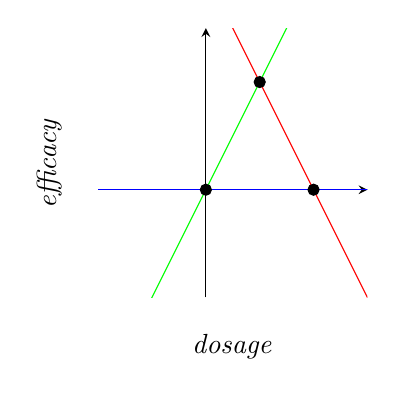
\begin{tikzpicture}
            \begin{axis}[
                axis lines=middle,
                width=5cm, height=5cm,
                xmin=-1, xmax=1.5,
                ymin=-1, ymax=1.5,
                x label style={at={(axis description cs:0.5,-0.1)},anchor=north},
                  y label style={at={(axis description cs:-0.1,.5)},rotate=90,anchor=south},
                xlabel={\textit{dosage}},
                ylabel={\textit{efficacy}},
                xtick=\empty, ytick=\empty
            ]
            \addplot [only marks] table {
                0 0.0
                0.5 1
                1  0   
                };
             \addplot+[no markers,green] {2*x};
             \addplot+[no markers,blue] {0*x};
             \addplot+[no markers,red] {-2*x + 2};
            \end{axis}
        \end{tikzpicture}
        
        Simple Regression can only fit 2 out of 3 points perfectly
    \column{0.49\textwidth}
        \begin{figure}
        \centering
        \includegraphics[trim={1cm 3cm 5cm 0.35cm },clip,width=\linewidth]{BP_4}
        \end{figure}
\end{columns}
\end{frame}

\begin{frame}[fragile]\frametitle{Recap: Neural Networks - Forward Pass}
\begin{columns}
    \column{0.5\textwidth}
        Example - Medical Study:
        \vspace{5mm}
        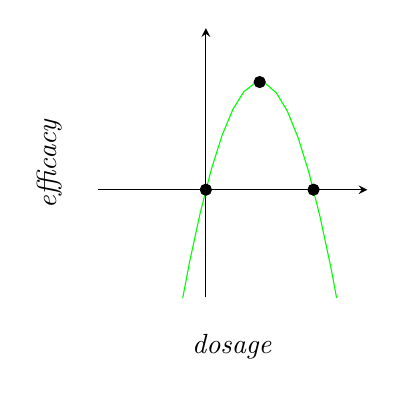
\begin{tikzpicture}
            \begin{axis}[
                samples=100,
                axis lines=middle,
                width=5cm, height=5cm,
                xmin=-1, xmax=1.5,
                ymin=-1, ymax=1.5,
                x label style={at={(axis description cs:0.5,-0.1)},anchor=north},
                  y label style={at={(axis description cs:-0.1,.5)},rotate=90,anchor=south},
                xlabel={\textit{dosage}},
                ylabel={\textit{efficacy}},
                xtick=\empty, ytick=\empty
            ]
            \addplot [only marks] table {
                0 0.0
                0.5 1
                1  0   
                };
            \addplot+[no markers,green] {3.91*sin(deg(x))+7.16*cos(deg(x))-7.16};
            \end{axis}
        \end{tikzpicture}
        
        A squiggle fits better! %(A periodic fit)
    \column{0.49\textwidth}
        \begin{figure}
        \centering
        \includegraphics[trim={1cm 3cm 5cm 0.35cm },clip,width=\linewidth]{BP_5}
        \end{figure}
\end{columns}
%  A trained network allows us to approximate for any new dosage
\pause
\begin{center}
    \Large \myblue{How to find values, so that the neural networks estimate the green squiggle? (Optimal Function Estimator)}
\end{center}
\end{frame}


\begin{frame}[fragile]\frametitle{Backpropagation - $b_3$}
\begin{columns}
    \column{0.5\textwidth}
    Assumption: Optimal parameters except $b_3$
    \column{0.49\textwidth}
        \begin{figure}
        \centering
        \includegraphics[trim={1cm 3cm 5cm 0.35cm },clip,width=\linewidth]{BP_6}
        \end{figure}
\end{columns}
\end{frame}

\begin{frame}[fragile]\frametitle{Backpropagation - $b_3$}
\begin{columns}
    \column{0.5\textwidth}
    Assumption: Optimal parameters given except $b_3$
    
    Backpropagation starts from back to front!
    
    Initialise $b_3 = 0$

       \vspace{5mm}
        \begin{tikzpicture}
            \begin{axis}[
                samples=100,
                axis lines=middle,
                width=5cm, height=5cm,
                xmin=-1, xmax=1.5,
                ymin=-3, ymax=1.5,
                x label style={at={(axis description cs:0.5,-0.1)},anchor=north},
                  y label style={at={(axis description cs:-0.1,.5)},rotate=90,anchor=south},
                xlabel={\textit{dosage}},
                ylabel={\textit{efficacy}},
                xtick=\empty, ytick=\empty
            ]
            \addplot [only marks] table {
                0 0.0
                0.5 1
                1  0   
                };
            \addplot+[no markers,green] {4.6*sin(deg(x))+7.3*cos(deg(x))-10.2};
            \end{axis}
        \end{tikzpicture}
    \column{0.49\textwidth}
        \begin{figure}
        \centering
        \includegraphics[trim={1cm 3cm 5cm 0.35cm },clip,width=\linewidth]{BP_7}
        \end{figure}
\end{columns}
%Since the bias sub 3 is now 0 it leaves it just to the sum and it is far away from the actual data.
\end{frame}

\begin{frame}[fragile]\frametitle{Backpropagation - $b_3=0$}
\begin{columns}
    \column{0.43\textwidth}
        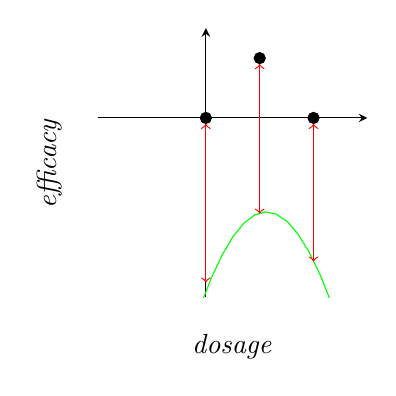
\begin{tikzpicture}
        \begin{axis}[
                samples=100,
                axis lines=middle,
                width=5cm, height=5cm,
                xmin=-1, xmax=1.5,
                ymin=-3, ymax=1.5,
                x label style={at={(axis description cs:0.5,-0.1)},anchor=north},
                  y label style={at={(axis description cs:-0.1,.5)},rotate=90,anchor=south},
                xlabel={\textit{dosage}},
                ylabel={\textit{efficacy}},
                xtick=\empty, ytick=\empty
            ]
            \addplot [only marks] table {
                0 0.0
                0.5 1
                1  0   
                };
            \addplot+[no markers,green] {4.6*sin(deg(x))+7.3*cos(deg(x))-10.2};
            \draw[<->,red] (axis cs:0,-0.1) -- (axis cs:0,-2.75);
            \draw[<->,red] (axis cs:0.5,0.9) -- (axis cs:0.5,-1.6);
            \draw[<->,red] (axis cs:1,-0.1) -- (axis cs:1,-2.4);
            \end{axis}
        \end{tikzpicture}
        
    \myblue{How large is the error?}\\\pause
    \textcolor{red}{Residual} = (Observed - Predicted)\\\pause
    $\textcolor{red}{R_1} = (0 - -2.6)$\\
    $\textcolor{red}{R_2} = (1 - -1.61)$\\
    $\textcolor{red}{R_3} = (0 - -2.61)$\\
    \myblue{What's the problem with the sum of these errors?}\pause

    \column{0.57\textwidth}
       Sum of squared residuals (SSR) to the rescue\\
       $\textcolor{red}{SSR} = (0 - -2.6)^2 + (1 - -1.61)^2 + (0 - -2.61)^2 = 20.4$\\
       For $b_3 = 0$

       \begin{tikzpicture}
        \begin{axis}[
                samples=100,
                axis lines=middle,
                width=5cm, height=5cm,
                xmin=-1, xmax=4.5,
                ymin=-0.2, ymax=22,
                x label style={at={(axis description cs:0.5,-0.1)},anchor=north},
                  y label style={at={(axis description cs:-0.1,.5)},rotate=90,anchor=south},
                xlabel={\textit{bias $b_3$}},
                ylabel={\textit{SSR}},
                xtick=\empty, ytick=\empty
            ]
            \addplot [only marks] table {
                0 20.4
                };
            \end{axis}
        \end{tikzpicture}
\end{columns}
\end{frame}

\begin{frame}[fragile]\frametitle{Backpropagation - $b_3=\{0,1,2,3\}$}
\begin{columns}
    \column{0.43\textwidth}
        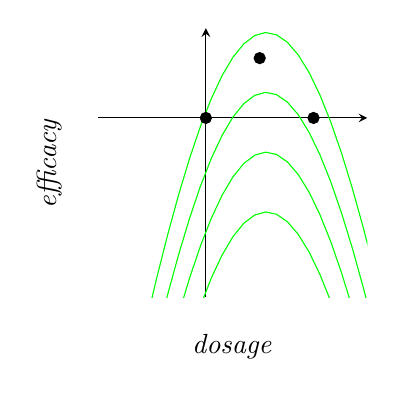
\begin{tikzpicture}
        \begin{axis}[
                samples=100,
                axis lines=middle,
                width=5cm, height=5cm,
                xmin=-1, xmax=1.5,
                ymin=-3, ymax=1.5,
                x label style={at={(axis description cs:0.5,-0.1)},anchor=north},
                  y label style={at={(axis description cs:-0.1,.5)},rotate=90,anchor=south},
                xlabel={\textit{dosage}},
                ylabel={\textit{efficacy}},
                xtick=\empty, ytick=\empty
            ]
            \addplot [only marks] table {
                0 0.0
                0.5 1
                1  0   
                };
            \addplot+[no markers,green] {4.6*sin(deg(x))+7.3*cos(deg(x))-10.2};
            \addplot+[no markers,green] {4.6*sin(deg(x))+7.3*cos(deg(x))-9.2};
            \addplot+[no markers,green] {4.6*sin(deg(x))+7.3*cos(deg(x))-8.2};
            \addplot+[no markers,green] {4.6*sin(deg(x))+7.3*cos(deg(x))-7.2};
            \end{axis}
        \end{tikzpicture}
    \column{0.57\textwidth}
    $\textcolor{red}{SSR_{b_3=0}} = (0 - -2.6)^2 + (1 - -1.61)^2 + (0 - -2.61)^2 = 20.4$\\
    $\textcolor{red}{SSR_{b_3=1}} = (0 - -1.6)^2 + (1 - -0.61)^2 + (0 - -1.61)^2 = 7.8$\\
    $\textcolor{red}{SSR_{b_3=2}} = (0 - -0.6)^2 + (1 - -0.39)^2 + (0 - -0.61)^2 = 1.1$\\
    $\textcolor{red}{SSR_{b_3=3}} =\qquad (0 - 0.04)^2 + (0 - 1.39)^2 + (0 - 0.39)^2 =  0.46$\\
    \vspace{2mm}
        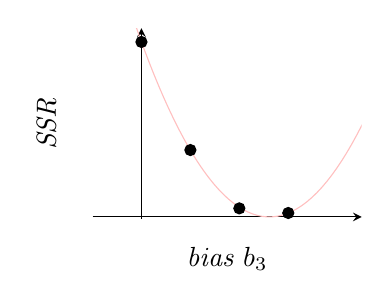
\begin{tikzpicture}
        \begin{axis}[
                samples=100,
                axis lines=middle,
                width=5cm, height=4cm,
                xmin=-1, xmax=4.5,
                ymin=-0.2, ymax=22,
                x label style={at={(axis description cs:0.5,-0.1)},anchor=north},
                  y label style={at={(axis description cs:-0.1,.5)},rotate=90,anchor=south},
                xlabel={\textit{bias $b_3$}},
                ylabel={\textit{SSR}},
                xtick=\empty, ytick=\empty
            ]
            \addplot [only marks] table {
                0 20.4
                1 7.8
                2 1. 1
                3 0.46
                };
                \addplot+[no markers,pink] {2.99*x^2 - 15.622*x + 20.408};
            \end{axis}
        \end{tikzpicture}
\end{columns}
\myred{Lowest point equals optimal $b_3$!}
\end{frame}

\begin{frame}[fragile]\frametitle{Backpropagation - Gradient Descent for $b_3$}
\begin{columns}
    \column{0.43\textwidth}
        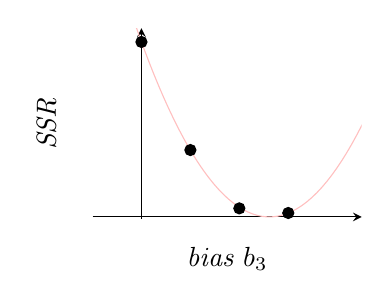
\begin{tikzpicture}
        \begin{axis}[
                samples=100,
                axis lines=middle,
                width=5cm, height=4cm,
                xmin=-1, xmax=4.5,
                ymin=-0.2, ymax=22,
                x label style={at={(axis description cs:0.5,-0.1)},anchor=north},
                  y label style={at={(axis description cs:-0.1,.5)},rotate=90,anchor=south},
                xlabel={\textit{bias $b_3$}},
                ylabel={\textit{SSR}},
                xtick=\empty, ytick=\empty
            ]
            \addplot [only marks] table {
                0 20.4
                1 7.8
                2 1. 1
                3 0.46
                };
                \addplot+[no markers,pink] {2.99*x^2 - 15.622*x + 20.408};
            \end{axis}
        \end{tikzpicture}\\

    To find the lowest point on the curve, use Gradient Descent to find the \textbf{derivative} of \myred{Sum of Squared Residuals} with respect to $b_3$\\
    \vspace{2mm}

    $SSR = \sum_{i=1}^{n=3} (\mathrm{Observed}_i - \textcolor{red}{\mathrm{Predicted}_i})^2$\\\pause

    \column{0.57\textwidth}
    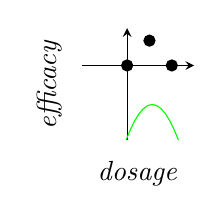
\begin{tikzpicture}
        \begin{axis}[
                samples=100,
                axis lines=middle,
                width=3cm, height=3cm,
                xmin=-1, xmax=1.5,
                ymin=-3, ymax=1.5,
                x label style={at={(axis description cs:0.5,-0.1)},anchor=north},
                  y label style={at={(axis description cs:-0.1,.5)},rotate=90,anchor=south},
                xlabel={\textit{dosage}},
                ylabel={\textit{efficacy}},
                xtick=\empty, ytick=\empty
            ]
            \addplot [only marks] table {
                0 0.0
                0.5 1
                1  0   
                };
            \addplot+[no markers,green] {4.6*sin(deg(x))+7.3*cos(deg(x))-10.2};
            \end{axis}
        \end{tikzpicture}

            $\mathrm{Predicted}_i = \textcolor{green}{\mathrm{green}_i}$ \pause $   = \textcolor{blue}{\mathrm{blue}_i} + \textcolor{orange}{\mathrm{orange}_i} + b_3$
            
    \begin{figure}
        \centering
        \includegraphics[trim={1cm 3cm 5cm 0.35cm },clip,width=\linewidth]{BP_5}
        \end{figure}
\end{columns}
\end{frame}

\begin{frame}[fragile]\frametitle{Backpropagation - Gradient Descent for $b_3$}
\begin{columns}
    \column{0.49\textwidth}
        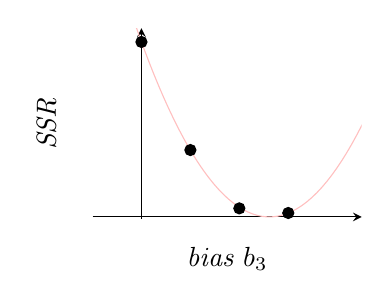
\begin{tikzpicture}
        \begin{axis}[
                samples=100,
                axis lines=middle,
                width=5cm, height=4cm,
                xmin=-1, xmax=4.5,
                ymin=-0.2, ymax=22,
                x label style={at={(axis description cs:0.5,-0.1)},anchor=north},
                  y label style={at={(axis description cs:-0.1,.5)},rotate=90,anchor=south},
                xlabel={\textit{bias $b_3$}},
                ylabel={\textit{SSR}},
                xtick=\empty, ytick=\empty
            ]
            \addplot [only marks] table {
                0 20.4
                1 7.8
                2 1. 1
                3 0.46
                };
                \addplot+[no markers,pink] {2.99*x^2 - 15.622*x + 20.408};
            \end{axis}
        \end{tikzpicture}\\

    \vspace{2mm}

    $SSR = \sum_{i=1}^{n=3} (\mathrm{Observed}_i - \mathrm{Predicted}_i)^2$\\
    
    \vspace{3mm}
    $\mathrm{Predicted}_i =  \textcolor{blue}{\mathrm{blue}_i} + \textcolor{orange}{\mathrm{orange}_i} + b_3$

    \vspace{3mm} 
    \textbf{Optimize SSR w.r.t. $b_3$ by gradient descent using the chain rule:} \pause  
    
    \vspace{3mm}
    $\displaystyle \frac{d SSR}{d b_3} =\textcolor{red}{ \frac{d SSR}{d \mathrm{Predicted}}} \times \displaystyle \frac{d \mathrm{Predicted}}{d b_3}$
    \pause
    \column{0.55\textwidth} 
    $\textcolor{red}{\displaystyle\frac{d SSR}{d \mathrm{Predicted}}} =$
    
    \vspace{3mm}
    \textbf{1st Substitute in the equation:}
    
    \vspace{3mm}
    $\displaystyle = \frac{d}{d \mathrm{Predicted}}  \sum_{i=1}^{n=3} (\mathrm{Observed}_i - \mathrm{Predicted}_i)^2$ \pause
    
    \vspace{3mm}
    \textbf{2nd Use chain rule:}
    
    \vspace{3mm}
    $\displaystyle =    \sum_{i=1}^{n=3} 2 \times (\mathrm{Observed}_i - \mathrm{Predicted}_i) \times -1$\pause

    \textbf{3rd Simplify:}
    
    \vspace{3mm}
    $\displaystyle =    \sum_{i=1}^{n=3} -2 \times (\mathrm{Observed}_i - \mathrm{Predicted}_i) $
    
\end{columns}
\end{frame}

\begin{frame}[fragile]\frametitle{Backpropagation - Gradient Descent for $b_3$}
\begin{columns}
    \column{0.49\textwidth}
        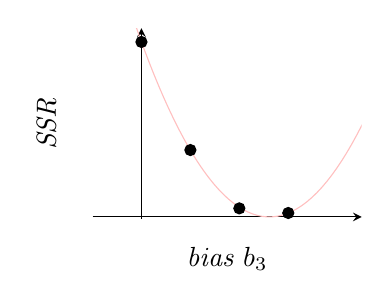
\begin{tikzpicture}
        \begin{axis}[
                samples=100,
                axis lines=middle,
                width=5cm, height=4cm,
                xmin=-1, xmax=4.5,
                ymin=-0.2, ymax=22,
                x label style={at={(axis description cs:0.5,-0.1)},anchor=north},
                  y label style={at={(axis description cs:-0.1,.5)},rotate=90,anchor=south},
                xlabel={\textit{bias $b_3$}},
                ylabel={\textit{SSR}},
                xtick=\empty, ytick=\empty
            ]
            \addplot [only marks] table {
                0 20.4
                1 7.8
                2 1. 1
                3 0.46
                };
                \addplot+[no markers,pink] {2.99*x^2 - 15.622*x + 20.408};
            \end{axis}
        \end{tikzpicture}\\

    \vspace{2mm}

    $SSR = \sum_{i=1}^{n=3} (\mathrm{Observed}_i - \mathrm{Predicted}_i)^2$\\
    
    \vspace{3mm}
    $\mathrm{Predicted}_i =  \textcolor{blue}{\mathrm{blue}_i} + \textcolor{orange}{\mathrm{orange}_i} + b_3$

    \vspace{3mm} 
    \textbf{Optimize SSR w.r.t. $b_3$ by gradient descent using the chain rule:} 
    
    \vspace{3mm}
    $\displaystyle \frac{d SSR}{d b_3} = \frac{d SSR}{d \mathrm{Predicted}} \times \textcolor{red}{\frac{d \mathrm{Predicted}}{d b_3}}$
    \pause
    \column{0.55\textwidth} 
    $\displaystyle \textcolor{red}{\frac{d \mathrm{Predicted}}{d b_3}} =$
    
    \vspace{3mm}
    \textbf{1st Substitute in the equation:}
    
    \vspace{3mm}
    $ = \frac{d}{d \mathrm{Predicted}}  \textcolor{blue}{\mathrm{blue}_i} + \textcolor{orange}{\mathrm{orange}_i} + b_3$ \pause
    
    \vspace{3mm}
    \textbf{2nd Derive:}
    
    \vspace{3mm}
    $\displaystyle =  0 + 0 + 1 = 1$

    
\end{columns}
\end{frame}

\begin{frame}[fragile]\frametitle{Backpropagation - Gradient Descent for $b_3$ - Final Derivative}
\begin{columns}
    \column{0.60\textwidth}
     
    $\displaystyle SSR = \sum_{i=1}^{n=3} (\mathrm{Observed}_i - \mathrm{Predicted}_i)^2$\\
    
    \vspace{3mm}
    $\displaystyle \mathrm{Predicted}_i =  \textcolor{blue}{\mathrm{blue}_i} + \textcolor{orange}{\mathrm{orange}_i} + b_3$

    \vspace{3mm} 
    
    $\displaystyle \frac{d SSR}{d \mathrm{Predicted}} =    \sum_{i=1}^{n=3} -2 \times (\mathrm{Observed}_i - \mathrm{Predicted}_i) $

    \vspace{3mm}
    $\displaystyle \frac{d SSR}{d \mathrm{Predicted}} = 1 $
    
    \vspace{5mm}
    $\displaystyle \frac{d SSR}{d b_3} = \frac{d SSR}{d \mathrm{Predicted}} \times \frac{d \mathrm{Predicted}}{d b_3}$
    \vspace{5mm}
   \textbf{ $\displaystyle \qquad \qquad=    \sum_{i=1}^{n=3} -2 \times (\mathrm{Observed}_i - \mathrm{Predicted}_i)\times 1$}

   \pause
    \column{0.39\textwidth} 

We can now plug in the observed and predicted values for each $b_3$ to determine the \textcolor{blue}{gradient} in the direction of the optimal $b_3$ value:

   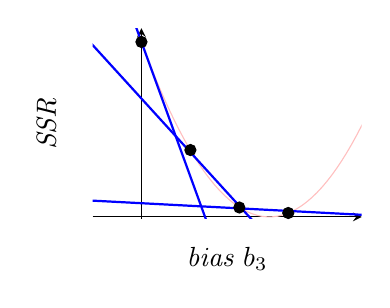
\begin{tikzpicture}
        \begin{axis}[
                samples=100,
                axis lines=middle,
                width=5cm, height=4cm,
                xmin=-1, xmax=4.5,
                ymin=-0.2, ymax=22,
                x label style={at={(axis description cs:0.5,-0.1)},anchor=north},
                  y label style={at={(axis description cs:-0.1,.5)},rotate=90,anchor=south},
                xlabel={\textit{bias $b_3$}},
                ylabel={\textit{SSR}},
                xtick=\empty, ytick=\empty
            ]
            \addplot [only marks] table {
                0 20.4
                1 7.8
                2 1.1
                3 0.46
                };
                \addplot+[no markers,pink] {2.99*x^2 - 15.622*x + 20.408};
                \addplot+[no markers,thick, blue] {-15.7*x+20.4};
                \addplot+[no markers,thick, blue] {-6.26*x+13.8};
                \addplot+[no markers,thick, blue] {-0.3*x+1.6};
            \end{axis}
        \end{tikzpicture}\\
\end{columns}
\end{frame}

\begin{frame}[fragile]\frametitle{Backpropagation - Gradient Descent for $b_3$ - Using the data}
\begin{columns}
    \column{0.60\textwidth}    
    $\displaystyle \frac{d SSR}{d b_3} =   \sum_{i=1}^{n=3} -2 \times (\mathrm{Observed}_i - \mathrm{Predicted}_i)\times 1$

    \vspace{3mm}
 
    For $b_3=0$:
    
    \vspace{3mm}
    
    $\displaystyle \frac{d SSR}{d b_3} = $
    
    $-2 \times (\mathrm{Observed}_1 - \mathrm{Predicted}_0)\times 1 +$
    $-2 \times (\mathrm{Observed}_2 - \mathrm{Predicted}_1)\times 1 +$
    $-2 \times (\mathrm{Observed}_3 - \mathrm{Predicted}_2)\times 1 =$
\pause
    \vspace{3mm}

    $-2 \times (0 - -2.6)\times 1 +$
    $-2 \times (1 - -1.6)\times 1 +$
    $-2 \times (0 - -2.61)\times 1 = -15.7$
\pause
    \vspace{3mm}

    $\mathrm{Step Size} = 0.1 \times -15.7 = -1.57$ (Learning Rate = 0.1)
    $\mathrm{New } b_3 = b_3 - \mathrm{Step Size} = 1.57$
    
    
    \column{0.39\textwidth} 
 \begin{tikzpicture}
        \begin{axis}[
                samples=100,
                axis lines=middle,
                width=5cm, height=5cm,
                xmin=-1, xmax=1.5,
                ymin=-3, ymax=1.5,
                x label style={at={(axis description cs:0.5,-0.1)},anchor=north},
                  y label style={at={(axis description cs:-0.1,.5)},rotate=90,anchor=south},
                xlabel={\textit{dosage}},
                ylabel={\textit{efficacy}},
                xtick=\empty, ytick=\empty
            ]
            \addplot [only marks] table {
                0 0.0
                0.5 1
                1  0   
                };
            \addplot+[no markers,green] {4.6*sin(deg(x))+7.3*cos(deg(x))-10.2};
         %   \addplot+[no markers,green] {4.6*sin(deg(x))+7.3*cos(deg(x))-9.2};
           % \addplot+[no markers,green] {4.6*sin(deg(x))+7.3*cos(deg(x))-8.2};
           % \addplot+[no markers,green] {4.6*sin(deg(x))+7.3*cos(deg(x))-7.2};
            \end{axis}
        \end{tikzpicture}
   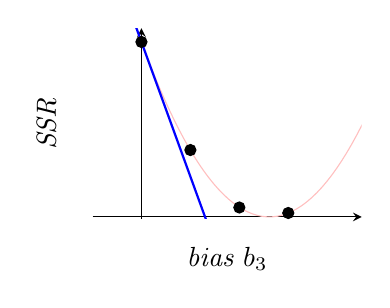
\begin{tikzpicture}
        \begin{axis}[
                samples=100,
                axis lines=middle,
                width=5cm, height=4cm,
                xmin=-1, xmax=4.5,
                ymin=-0.2, ymax=22,
                x label style={at={(axis description cs:0.5,-0.1)},anchor=north},
                  y label style={at={(axis description cs:-0.1,.5)},rotate=90,anchor=south},
                xlabel={\textit{bias $b_3$}},
                ylabel={\textit{SSR}},
                xtick=\empty, ytick=\empty
            ]
            \addplot [only marks] table {
                0 20.4
                1 7.8
                2 1.1
                3 0.46
                };
                \addplot+[no markers,pink] {2.99*x^2 - 15.622*x + 20.408};
                \addplot+[no markers,thick, blue] {-15.7*x+20.4};
            \end{axis}
        \end{tikzpicture}\\
\end{columns}
\end{frame}

\begin{frame}[fragile]\frametitle{Backpropagation - Gradient Descent for $b_3$ - Using the data}
\begin{columns}
    \column{0.60\textwidth}    
    $\displaystyle \frac{d SSR}{d b_3} =   \sum_{i=1}^{n=3} -2 \times (\mathrm{Observed}_i - \mathrm{Predicted}_i)\times 1$

    \vspace{3mm}
 
    For $b_3=1.57$:
    
    \vspace{3mm}
    
    $\displaystyle \frac{d SSR}{d b_3} = $
    
    $-2 \times (\mathrm{Observed}_1 - \mathrm{Predicted}_0)\times 1 +$
    $-2 \times (\mathrm{Observed}_2 - \mathrm{Predicted}_1)\times 1 +$
    $-2 \times (\mathrm{Observed}_3 - \mathrm{Predicted}_2)\times 1 =$
    \vspace{3mm}

    $-2 \times (0 - -1.03)\times 1 +$
    $-2 \times (1 - -0.03)\times 1 +$
    $-2 \times (0 - -1.04)\times 1 = -6.26$
    \vspace{3mm}

    $\mathrm{Step Size} = 0.1 \times -6.26 = -0.62$ (Learning Rate = 0.1)
    $\mathrm{New } b_3 = b_3 - \mathrm{Step Size} = 2.19$ 
    
    
    \column{0.39\textwidth} 
 \begin{tikzpicture}
        \begin{axis}[
                samples=100,
                axis lines=middle,
                width=5cm, height=5cm,
                xmin=-1, xmax=1.5,
                ymin=-3, ymax=1.5,
                x label style={at={(axis description cs:0.5,-0.1)},anchor=north},
                  y label style={at={(axis description cs:-0.1,.5)},rotate=90,anchor=south},
                xlabel={\textit{dosage}},
                ylabel={\textit{efficacy}},
                xtick=\empty, ytick=\empty
            ]
            \addplot [only marks] table {
                0 0.0
                0.5 1
                1  0   
                };
           % \addplot+[no markers,green] {4.6*sin(deg(x))+7.3*cos(deg(x))-10.2};
            \addplot+[no markers,green] {4.6*sin(deg(x))+7.3*cos(deg(x))-9.2};
            %\addplot+[no markers,green] {4.6*sin(deg(x))+7.3*cos(deg(x))-8.2};
           % \addplot+[no markers,green] {4.6*sin(deg(x))+7.3*cos(deg(x))-7.2};
            \end{axis}
        \end{tikzpicture}
   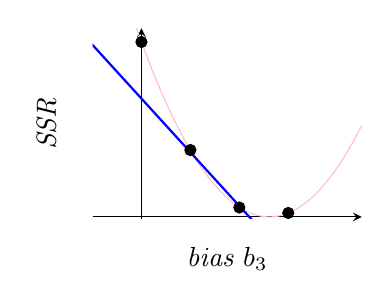
\begin{tikzpicture}
        \begin{axis}[
                samples=100,
                axis lines=middle,
                width=5cm, height=4cm,
                xmin=-1, xmax=4.5,
                ymin=-0.2, ymax=22,
                x label style={at={(axis description cs:0.5,-0.1)},anchor=north},
                  y label style={at={(axis description cs:-0.1,.5)},rotate=90,anchor=south},
                xlabel={\textit{bias $b_3$}},
                ylabel={\textit{SSR}},
                xtick=\empty, ytick=\empty
            ]
            \addplot [only marks] table {
                0 20.4
                1 7.8
                2 1.1
                3 0.46
                };
                \addplot+[no markers,pink] {2.99*x^2 - 15.622*x + 20.408};
                \addplot+[no markers,thick, blue] {-6.26*x+13.8};
                %\addplot+[no markers,thick, blue] {-0.3*x+1.6};
            \end{axis}
        \end{tikzpicture}\\
\end{columns}
\end{frame}

\begin{frame}[fragile]\frametitle{Backpropagation - Gradient Descent for $b_3$ - Using the data \textit{very often}}
\begin{columns}
    \column{0.60\textwidth}    
    $\displaystyle \frac{d SSR}{d b_3} =   \sum_{i=1}^{n=3} -2 \times (\mathrm{Observed}_i - \mathrm{Predicted}_i)\times 1$

    \vspace{3mm}
 
    For $b_3=2.61$:
    
    \vspace{3mm}
    
    $\displaystyle \frac{d SSR}{d b_3} = $
    
    $-2 \times (\mathrm{Observed}_1 - \mathrm{Predicted}_0)\times 1 +$
    $-2 \times (\mathrm{Observed}_2 - \mathrm{Predicted}_1)\times 1 +$
    $-2 \times (\mathrm{Observed}_3 - \mathrm{Predicted}_2)\times 1 \approx$
    \vspace{3mm}

    $-2 \times (0 - 0.01)\times 1 +$
    $-2 \times (1 - 1.01)\times 1 +$
    $-2 \times (0 - 0)\times 1 \approx 0$
    \vspace{3mm}

    $\mathrm{Step Size} = 0.1 \times 0 = 0$ (Learning Rate = 0.1)
    $\mathrm{New } b_3 = b_3 - \mathrm{Step Size} = \textbf{2.61}$
    
    
    \column{0.39\textwidth} 
 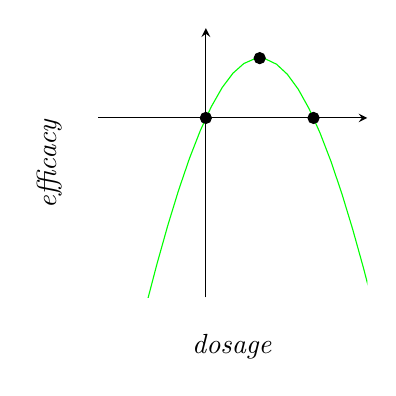
\begin{tikzpicture}
        \begin{axis}[
                samples=100,
                axis lines=middle,
                width=5cm, height=5cm,
                xmin=-1, xmax=1.5,
                ymin=-3, ymax=1.5,
                x label style={at={(axis description cs:0.5,-0.1)},anchor=north},
                  y label style={at={(axis description cs:-0.1,.5)},rotate=90,anchor=south},
                xlabel={\textit{dosage}},
                ylabel={\textit{efficacy}},
                xtick=\empty, ytick=\empty
            ]
            \addplot [only marks] table {
                0 0.0
                0.5 1
                1  0   
                };
           % \addplot+[no markers,green] {4.6*sin(deg(x))+7.3*cos(deg(x))-10.2};
           % \addplot+[no markers,green] {4.6*sin(deg(x))+7.3*cos(deg(x))-9.2};
           % \addplot+[no markers,green] {4.6*sin(deg(x))+7.3*cos(deg(x))-8.2};
            \addplot+[no markers,green] {3.91*sin(deg(x))+7.16*cos(deg(x))-7.16};
            \end{axis}
        \end{tikzpicture}
   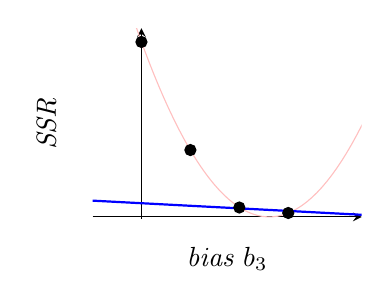
\begin{tikzpicture}
        \begin{axis}[
                samples=100,
                axis lines=middle,
                width=5cm, height=4cm,
                xmin=-1, xmax=4.5,
                ymin=-0.2, ymax=22,
                x label style={at={(axis description cs:0.5,-0.1)},anchor=north},
                  y label style={at={(axis description cs:-0.1,.5)},rotate=90,anchor=south},
                xlabel={\textit{bias $b_3$}},
                ylabel={\textit{SSR}},
                xtick=\empty, ytick=\empty
            ]
            \addplot [only marks] table {
                0 20.4
                1 7.8
                2 1.1
                3 0.46
                };
                \addplot+[no markers,pink] {2.99*x^2 - 15.622*x + 20.408};
                %\addplot+[no markers,thick, blue] {-6.26*x+13.8};
                \addplot+[no markers,thick, blue] {-0.3*x+1.6};
            \end{axis}
        \end{tikzpicture}
\end{columns}
\end{frame}

\begin{frame}[fragile]\frametitle{Summary - Backpropagation}
\begin{columns}
    \column{0.59\textwidth} 

     The main ideas of backpropagation are that when a parameter is unknown, like $b_3$, we use the \textbf{chain rule} to calculate the derivative of \textbf{sum of the squared residuals (SSR)} with respect to the unknown parameters.

     Then we initialize the unknown parameter and use \textbf{Gradient Descent} to optimize the unknown parameter, here $b_3$.
     
    \begin{figure}
    \centering
    \includegraphics[trim={1cm 3cm 5cm 0.35cm },clip,width=0.75\linewidth]{BP_6}
    \end{figure}
    
    \column{0.39\textwidth} 
 
    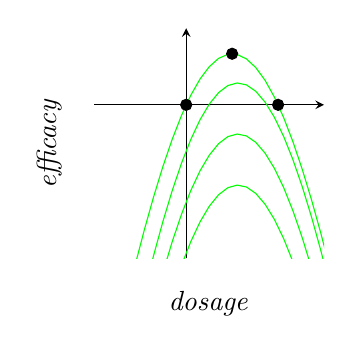
\begin{tikzpicture}
        \begin{axis}[
                samples=100,
                axis lines=middle,
                width=4.5cm, height=4.5cm,
                xmin=-1, xmax=1.5,
                ymin=-3, ymax=1.5,
                x label style={at={(axis description cs:0.5,-0.1)},anchor=north},
                  y label style={at={(axis description cs:-0.1,.5)},rotate=90,anchor=south},
                xlabel={\textit{dosage}},
                ylabel={\textit{efficacy}},
                xtick=\empty, ytick=\empty
            ]
            \addplot [only marks] table {
                0 0.0
                0.5 1
                1  0   
                };
            \addplot+[no markers,green] {4.6*sin(deg(x))+7.3*cos(deg(x))-10.2};
            \addplot+[no markers,green] {4.6*sin(deg(x))+7.3*cos(deg(x))-9.2};
            \addplot+[no markers,green] {4.6*sin(deg(x))+7.3*cos(deg(x))-8.2};
            \addplot+[no markers,green] {3.91*sin(deg(x))+7.16*cos(deg(x))-7.16};
            \end{axis}
        \end{tikzpicture}
   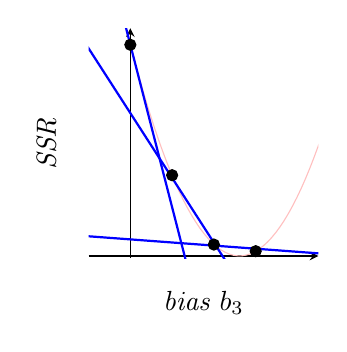
\begin{tikzpicture}
        \begin{axis}[
                samples=100,
                axis lines=middle,
                width=4.5cm, height=4.5cm,
                xmin=-1, xmax=4.5,
                ymin=-0.2, ymax=22,
                x label style={at={(axis description cs:0.5,-0.1)},anchor=north},
                  y label style={at={(axis description cs:-0.1,.5)},rotate=90,anchor=south},
                xlabel={\textit{bias $b_3$}},
                ylabel={\textit{SSR}},
                xtick=\empty, ytick=\empty
            ]
            \addplot [only marks] table {
                0 20.4
                1 7.8
                2 1.1
                3 0.46
                };
                \addplot+[no markers,pink] {2.99*x^2 - 15.622*x + 20.408};
                \addplot+[no markers,thick, blue] {-15.7*x+20.4};
                \addplot+[no markers,thick, blue] {-6.26*x+13.8};
                \addplot+[no markers,thick, blue] {-0.3*x+1.6};
            \end{axis}
        \end{tikzpicture}\\
\end{columns}
\end{frame}

\begin{frame}\frametitle{Backpropagation - Notes}
\begin{itemize}
    \item Backpropagation: A method used to calculate gradients in a neural network to improve weights and biases given a loss function. 
    \item Note: Backpropagation refers only to the method for computing the gradient, while another algorithm, such as gradient descent, is used to perform learning using this gradient.
    \item Intuituion: Derived from the fact that the method starts the process at the output layer, and works towards the input layer, propagating the error-induced changes backward throughout the network. 
    \item Learning Rate: Tuning parameter determing the step size at each iteration while moving toward a minimum of a loss function.
    \item Loss Function: A function that maps an event (input-output-pair) onto a real number representing some "cost" associated with the event. The goal of (machine) learning is to minimize the loss.
    \item Chain Rule: $\displaystyle [f(g(x))]'=f'(g(x))\cdot g'(x)$
\end{itemize}
\end{frame}

\begin{frame}{Take-Away and Outlook} 
What have we learned?
\begin{itemize}
    \item Main Ideas for Backpropagation
\end{itemize}
What do we do next time?
\begin{itemize}
    \item Calculating all parameters at the same time using the chain rule and matrix multiplication
    \item Stochastic Gradient Descent %(randomly selected subset of the dataset to reduce time)
    \item Optimization Algorithms, Learning Rate
    \item Computational Graph (PyTorch)
\end{itemize}
Reading Material:
\begin{itemize}
    \item Goodfellow, Ian, Yoshua Bengio, and Aaron Courville. Deep learning. MIT press, 2016. The chapter on Backpropagation.
\end{itemize}
\end{frame}


%%%% REFERENZEN %%%%
\begin{frame}\frametitle{References}
\begin{itemize}
    \item Goodfellow, Ian, Yoshua Bengio, and Aaron Courville. Deep learning. MIT press, 2016.
    \item Demystifying Deep Neural Net by Rosie Campbell \url{https://medium.com/@RosieCampbell/demystifying-deep-neural-nets-efb726eae941}
    \item Step-by-step neural network and backpropagation IPython Notebook by Andrew Trask: \url{https://tinyurl.com/Grokking-Deep-Learning-Cha-6}
    \item Well-written Python implementation by Matt Mazur \url{https://github.com/mattm/simple-neural-network} and the according blog post \url{https://mattmazur.com/2015/03/17/a-step-by-step-backpropagation-example/}
    \item Slides are based on a video by StatQuest with Josh Starmer about the Chain Rule \url{https://youtu.be/wl1myxrtQHQ}, and about Neural Networks \url{https://youtu.be/CqOfi41LfDw} 
\end{itemize}
\end{frame}


\begin{frame}{\textbf{Thank you for your \textbf{attention}!}}
    \begin{columns}
	\column{.59\textwidth}
	 \begin{center}
        \small{\faGraduationCap \hspace{0.15em} {Resources (Slides, Self-tests, exercises, link to Jupyter Notebooks...)\\\small{\faGithub \hspace{0.15em} {\href{https://github.com/RicardoUsbeck/BP}{https://github.com/RicardoUsbeck/BP}}}}} \\
        \smallskip
        \Huge {Which questions do you have?} \\
        
    \end{center}
	\column{.4\textwidth}
	\centering
	\includegraphics[width=0.65\linewidth]{Geoffrey_Hinton_at_UBC.jpg}\\
	
	\vspace{3mm}
	
	\tiny \textcolor{gray}{Geoffrey Hinton - ACM A. M. Turing Award Winner for conceptual and engineering breakthroughs that have made deep neural networks a critical component of computing. Source: Eviatar Bach (\url{commons.wikimedia.org/wiki/File:Geoffrey_Hinton_at_UBC.jpg}), „Geoffrey Hinton at UBC“, \url{creativecommons.org/licenses/by-sa/3.0/legalcode}}

\end{columns}
\end{frame}

%For Deeper Networks: Matrix Multiplication
%Given an input–output pair {\displaystyle (x,y)}(x,y), the loss is:

%{\displaystyle C(y,f^{L}(W^{L}f^{L-1}(W^{L-1}\cdots f^{2}(W^{2}f^{1}(W^{1}x))\cdots )))}{\displaystyle C(y,f^{L}(W^{L}f^{L-1}(W^{L-1}\cdots f^{2}(W^{2}f^{1}(W^{1}x))\cdots )))}
%To compute this, one starts with the input {\displaystyle x}x and works forward; denote the weighted input of each hidden layer as {\displaystyle z^{l}}{\displaystyle z^{l}} and the output of hidden layer {\displaystyle l}l as the activation {\displaystyle a^{l}}{\displaystyle a^{l}}. For backpropagation, the activation {\displaystyle a^{l}}{\displaystyle a^{l}} as well as the derivatives {\displaystyle (f^{l})'}{\displaystyle (f^{l})'} (evaluated at {\displaystyle z^{l}}{\displaystyle z^{l}}) must be cached for use during the backwards pass.

%The derivative of the loss in terms of the inputs is given by the chain rule; note that each term is a total derivative, evaluated at the value of the network (at each node) on the input {\displaystyle x}x:

%{\displaystyle {\frac {dC}{da^{L}}}\circ {\frac {da^{L}}{dz^{L}}}\cdot {\frac {dz^{L}}{da^{L-1}}}\circ {\frac {da^{L-1}}{dz^{L-1}}}\cdot {\frac {dz^{L-1}}{da^{L-2}}}\circ \ldots \circ {\frac {da^{1}}{dz^{1}}}\cdot {\frac {\partial z^{1}}{\partial x}},}{\displaystyle {\frac {dC}{da^{L}}}\circ {\frac {da^{L}}{dz^{L}}}\cdot {\frac {dz^{L}}{da^{L-1}}}\circ {\frac {da^{L-1}}{dz^{L-1}}}\cdot {\frac {dz^{L-1}}{da^{L-2}}}\circ \ldots \circ {\frac {da^{1}}{dz^{1}}}\cdot {\frac {\partial z^{1}}{\partial x}},}
%where {\displaystyle \circ }\circ  is a Hadamard product, that is an element-wise product.

%These terms are: the derivative of the loss function;[d] the derivatives of the activation functions;[e] and the matrices of weights:[f]

%{\displaystyle {\frac {dC}{da^{L}}}\circ (f^{L})'\cdot W^{L}\circ (f^{L-1})'\cdot W^{L-1}\circ \cdots \circ (f^{1})'\cdot W^{1}.}{\displaystyle {\frac {dC}{da^{L}}}\circ (f^{L})'\cdot W^{L}\circ (f^{L-1})'\cdot W^{L-1}\circ \cdots \circ (f^{1})'\cdot W^{1}.}
%The gradient {\displaystyle \nabla }\nabla  is the transpose of the derivative of the output in terms of the input, so the matrices are transposed and the order of multiplication is reversed, but the entries are the same:

%{\displaystyle \nabla _{x}C=(W^{1})^{T}\cdot (f^{1})'\circ \ldots \circ (W^{L-1})^{T}\cdot (f^{L-1})'\circ (W^{L})^{T}\cdot (f^{L})'\circ \nabla _{a^{L}}C.}{\displaystyle \nabla _{x}C=(W^{1})^{T}\cdot (f^{1})'\circ \ldots \circ (W^{L-1})^{T}\cdot (f^{L-1})'\circ (W^{L})^{T}\cdot (f^{L})'\circ \nabla _{a^{L}}C.}


\end{document}
